                        [104 v\textsuperscript{o}]  etiam 
                        alius super alium spatio inter eos relicto  poterit suspendi. Porro 
           %              \begin{wrapfigure}{l}{0.25\textwidth}                    
               % 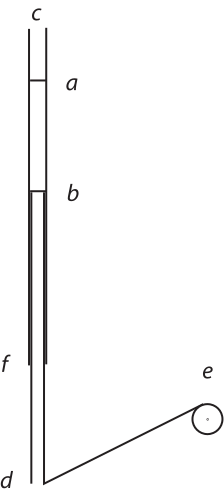
\includegraphics[width=0.25\textwidth]{images/37_3_104v}\\\textit{[Fig. 5]}
                        %\caption{Bildbeschreibung}
                   %     \end{wrapfigure}
                        %@ @ @ Dies ist eine Abstandszeile - fuer den Fall, dass mehrere figures hintereinander kommen, ohne dass dazwischen laengerer Text steht. Dies kann zu einer Fahlermeldung fuehren. @ @ @ \\
                        notabile est  si Mercurio\protect\index{Sachverzeichnis}{mercurius} suspenso continuo, in infinitum, affundas  novum, aut adimas priorem;\footnote{\textit{In der rechten Spalte}: \textso{Exp. 19.}} summum  punctum suspensionis nihilominus nunquam nec descensurum  nec ascensurum, sed fixum mansurum. Ratio  est quia quantum superfunditur tantum deprimitur,  quantum aufertur, tantum attollitur. \edtext{Quod illustrari}{\lemma{Quod}\Afootnote{ \textit{ (1) }\ clarius intelligi \textit{ (2) }\ illustrari \textit{ L}}} poterit experimento in Elaterio\protect\index{Sachverzeichnis}{elaterium} simplici capto, ex quo apparebit  liquorem non minus contra eundem liquorem, quam contra Elaterium\protect\index{Sachverzeichnis}{elaterium} aliquod ex eadem semper altitudine ponderare. Esto \edtext{[\textit{[Fig. 5]}]}{\lemma{}\Afootnote{fig. 3\textit{\ L \"{a}ndert Hrsg. }\ fig. 3 \textit{ erg.} \textit{ L }}} Mercurius\protect\index{Sachverzeichnis}{mercurius} \textit{ab} in Tubo \textit{cf} premens Embolum\protect\index{Sachverzeichnis}{embolus}  
% Zeitzauskommentiert                       \begin{wrapfigure}{l}{0.27\textwidth}                    
%                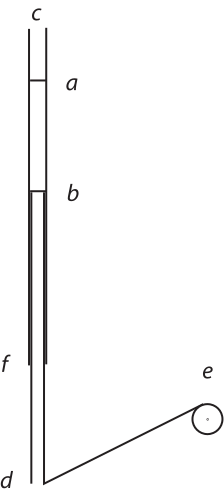
\includegraphics[width=0.27\textwidth]{images/37_3_104v}\\\textit{[Fig. 5]}
%                        %\caption{Bildbeschreibung}
%                        \end{wrapfigure}    
                        exacte tubo aptatum \textit{bd} embolum\protect\index{Sachverzeichnis}{embolus} autem  per chordam cum rota \textit{e} communicare, 
                                                eamque  descendendo circumagere, et hac circumactione Elaterium\protect\index{Sachverzeichnis}{elaterium} quoddam tendere. Observetur \edtext{punctum summum}{\lemma{}\Afootnote{punctum summum \textit{ erg.} \textit{ L}}} altitudinis  ultra quam Mercurius\protect\index{Sachverzeichnis}{mercurius} descendere seu Elaterium\protect\index{Sachverzeichnis}{elaterium}  porro comprimere non potest nempe \textit{a}.  Infundatur plus Mercurii\protect\index{Sachverzeichnis}{mercurius}, tantundem semper quantum  infundes descendet, \edtext{et embolum\protect\index{Sachverzeichnis}{embolus} deprimet, et Elaterium\protect\index{Sachverzeichnis}{elaterium} porro tendet,}{\lemma{}\Afootnote{et [...] tendet, \textit{ erg.} \textit{ L}}} at nihilominus summum Mercurii\protect\index{Sachverzeichnis}{mercurius}  punctum semper manebit \textit{a}. Cum enim Elaterium\protect\index{Sachverzeichnis}{elaterium}  sustineat \textit{ab} id semper  sustinebit, additum autem rem suam aget solum,  quippe nulla resistentia destructum, quam Elaterium\protect\index{Sachverzeichnis}{elaterium}  in \textit{ab} sustinendum totam consumit.\footnote{\textit{In der rechten Spalte}: At caetera phaenomena Gravitati aeris communiter ascripta.} 
                        %Afootnote zu footnote, muss noch an richtige Stelle geschoben werden, hängt aber von Seitenaufteilung vorher ab.                
                         Ergo  quicquid ultra \textit{ab} additur semper sine resistentia  descendet Elateriumque\protect\index{Sachverzeichnis}{elaterium} tendet. Similiter si ex \textit{ab}  adimas, tantundem sursum pelletur ab Elaterii\protect\index{Sachverzeichnis}{elaterium}  renisu, sed nunquam ultra \textit{a}. Quare toto Mercurii\protect\index{Sachverzeichnis}{mercurius}  pondere ablato, Elaterium\protect\index{Sachverzeichnis}{elaterium} non attollet Embolum\protect\index{Sachverzeichnis}{embolus}  ultra \textit{a}. Hinc elegans propositio conficitur liquorem Elaterium\protect\index{Sachverzeichnis}{elaterium} comprimentem nunquam descendere infra  altitudinem in quam ipsum Elaterium\protect\index{Sachverzeichnis}{elaterium} assurgit  non \edtext{compressum, scilicet}{\lemma{compressum,~\textbar\ seu}\Afootnote{ut liquores ita Elateria\protect\index{Sachverzeichnis}{elaterium} quoque  determinatam altitudinem servare \textit{ gestr.}~\textbar\ ~scilicet \textit{ L}}} si Elaterium\protect\index{Sachverzeichnis}{elaterium} ipsum sit liquidum, ut aer, ubi crassities  tubi \textit{af} nihil ad rem facit, ut constat ex aequipondio  liquorum. Hinc ut in Elaterio\protect\index{Sachverzeichnis}{elaterium} sicco res succedat, liquor \textit{ab} aut ejus loco pondus quodcunque \edtext{cylindricum}{\lemma{cylindricum}\Afootnote{\textit{ erg.} \textit{ L}}} premens non debet  esse latius quam ut \edtext{premendo}{\lemma{premendo}\Afootnote{\textit{ erg.} \textit{ L}}}   
                         %Afootnote zu Footnote von oben
                               \edtext{}{\lemma{phaenomena}\linenum{|26|||26|}\Afootnote{ \textit{ (1) }\ pressioni \textit{ (2) }\ Gravitati \textit{ L}}}
                              descendat praecise infra \textit{a} non  ultra. Et haec latitudo semel determinata  semper servanda est, altitudine tantum addendo  ad pondus demendove variata. At pro comprimendis Elateriis\protect\index{Sachverzeichnis}{elaterium} liquidis non est opus hac cautione. Ut  in aere Baroscopium\protect\index{Sachverzeichnis}{baroscopium} commune, imo et Tubus utrinque  clausus manifeste confirmant.\pend \pstart  Ex his determinatae in Baroscopio\protect\index{Sachverzeichnis}{baroscopium}  altitudinis causam satis \edtext{apparere}{\lemma{satis}\Afootnote{ \textit{ (1) }\ detectam \textit{ (2) }\ apparere \textit{ L}}} puto, quia \edtext{gravitati columnae aereae,}{\lemma{quia}\Afootnote{ \textit{ (1) }\ scilicet aeris columnae, \textit{ (2) }\ gravitati columnae aereae, \textit{ L}}} aut  huic aequali aeris resistentiae ad ulteriorem compressionem  aequiponderat. Hinc jam in aere compresso necesse \edtext{est Baroscopium}{\lemma{est}\Afootnote{ \textit{ (1) }\ aeris \textit{ (2) }\ Baroscopium \textit{ L}}} esse altius, et in rarefacto depressius. 
                             \pend 
% Zeitz auskommentiert                             % \clearpage
%                       \begin{center}                 
%                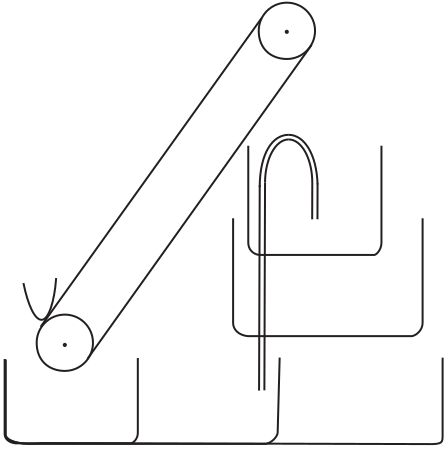
\includegraphics[width=0.3\textwidth]{images/37_3_103r2}\\\textit{[Fig. 6, Bleistiftzeichnung, nicht zuzuordnen]}
%                        %\caption{Bildbeschreibung}
%                        \end{center}
%                        %@ @ @ Dies ist eine Abstandszeile - fuer den Fall, dass mehrere figures hintereinander kommen, ohne dass dazwischen laengerer Text steht. Dies kann zu einer Fahlermeldung fuehren. @ @ @ \\
                    